\section{Method}
In order to answer the research questions stated in section~\ref{sec:RQ} a state of the art SPC, experiments and evaluation methods needs to be set up. In this section the SPC hardware and image sensing and reconstruction scheme is described as well as the different evaluation metrics and methods.


\subsection{Single pixel camera architecture and hardware}
\label{sec:system}
FOI designed the SWIR SPC platform using a DMD, a Newtonian telescope and a single pixel detector which are further described in section~\ref{sec:hardware}. The system also has a reference camera in the visual spectrum  which can capture images if all micro mirrors in the DMD are turned away from the single pixel sensor and towards the reference camera, it can also be used to check that the patterns are displayed correct.  

\begin{figure}[H]
    \centering
    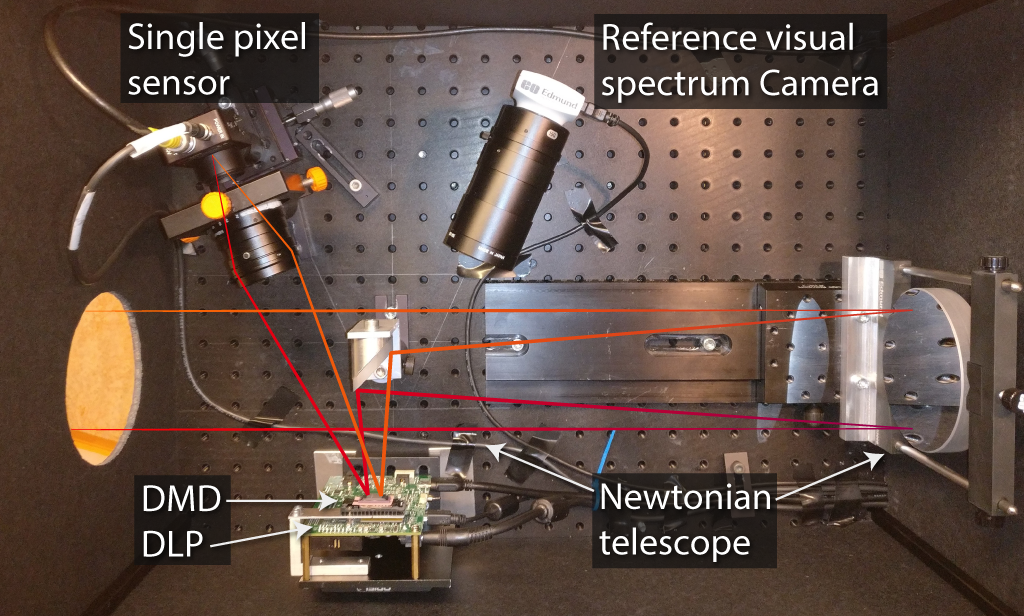
\includegraphics[width = 0.8\textwidth]{gfx/SPC.png}
    \caption{Single pixel imaging system (SPIS), adopted from \cite{article:foiSPIS}.}
    \label{fig:system1}
\end{figure}



As seen in figure~\ref{fig:system1} light from the scene is focused by the Newtonian telescope and reflected onto the DMD. The mirrors on the DMD can turned individually either into the single pixel sensor or the reference camera. The DMD acts as a Spatial Light Modulator (SLM) and reflects different patterns which is 'summed up' in the single pixel sensor as an intensity. The reconstructed image from the system will have the same resolution as the DMD patterns. The DLP is the DMD control unit which controls which patterns that are displayed on the DMD either by reading images from memory or the video port.   

\subsubsection{Hardware}
\label{sec:hardware}
\subsubsection{Newtonian telescope}
A Newtonian telescope is a reflecting telescope, using a concave primary mirror and a flat diagonal secondary mirror, see figure~\ref{fig:system1}. In this set-up the telescope act as a lens focusing the scene onto the DMD. The motivation to use a Newtonian telescope instead of a lens system is partly that chromatic aberration is eliminated and partly that a reflective optical system works over a greater range of wavelengths that includes SWIR, near infrared (NIR) and the visible spectrum.

\subsubsection{DLP and DMD}
The DMD (Texas Instruments DLP4500NIR) is a matrix of micro mirrors that can be individually tilted $\pm 12^{\circ}$ and reflects wavelengths in the range 700-2500 nm. The DMD is controlled by the DLP (DLP LightCrafter 4500) which can be controlled either by video port (HDMI) or by the internal flash memory. The internal memory can theoretically be faster then the video port but due to constraints in both memory and memory bandwidth the fastest measurement matrix rate gets stuck at $270 - 300$ Hz. The video port can be operated at 120 Hz and display one bit plane at the time, which gives a maximum measurement matrix rate at $120 * 24 = 2880$ Hz, but in the current configuration only $60$ Hz frame rate was achieved giving a measurement matrix rate at $1440$ Hz.  


Because the diamond shape of the mirrors and how their index is defined in the DLP where one column is two mirror column arrays wide, see figure~\ref{fig:dmd_index}, the reconstructed image needs to be reshaped to a Cartesian grid. To control the DMD the software 'DLP LightCrafter 4500 Control Software' is used. \cite{manual:DLP}


\begin{figure}[H]
    \centering
    
\includegraphics[width = 0.8\textwidth]{gfx/DMD_grid.png}
    \caption{DMD matrix, left shows each tiles index and right shows second row and second column in black.}
    \label{fig:dmd_index}
\end{figure}

\begin{figure}[H]
    \centering
    
\includegraphics[width = 0.8\textwidth]{gfx/DMD_grid2.png}
    \caption{DMD matrix, left shows each tiles index and right shows second row and second column in black.}
    \label{fig:dmd_index2}
\end{figure}


How does this effect the result?

\subsubsection{Lens}
The lens mounted on the single pixel sensor is an 50mm SWIR Fixed Focal Length Lens f1.4 designed for wavelengths raging from the 800 nm in the visual spectrum to 2000 nm in the SWIR spectrum. \cite{website:SWIR_objective}

\subsubsection{Single pixel sensor}
The single pixel sensor is a Thorlabs PDA20C/M and is sensitive in wavelength range 800-1700 nm which is beyond the visual spectrum (390-700 nm). \cite{manual:PDA}

\subsubsection{Signal spectrum}
All components characteristics assembled should capture signals in 800-1700 nm spectrum.



\subsection{System overview}

\subsubsection{Measurement matrix}

\subsubsection{Reconstruction algorithm}

\subsection{Evaluation}
The evaluation will be divided in to two categories: reconstructed images from synthetic data and images reconstructed from data acquired by the SPC.\\[0.1in] 

The evaluation on synthetic data is focused on evaluating the performance of the measurement matrix and reconstruction algorithm. Evaluating synthetic data gives two possibilities that can not be achieved with images reconstructed using the SPC which is that there is a reference image which the resulting image can be compared to.

Reconstructed image from synthetic data is acquired by creating a signal $ \mathbf{ y }_{M\times1}$ taking the inner product of $ \mathbf{y} = \mathbf{\Phi} \mathbf{x} + \epsilon$ where, $\mathbf{x}$ is the synthetic image reshaped to a vector, $\mathbf{\Phi}$ is the measurement matrix with the desired amount of measurements $M$ and synthetic noise $\epsilon$ which can be regulated to simulate different conditions, then using the reconstruction algorithm on the signal $\mathbf{y}$ to obtain the reconstructed image $\mathbf{\hat x}$. Because the measurement matrix and reconstruction algorithm is independent of the SPC hardware the subsystem can be evaluated independently. Two advantages of evaluation the sensing and reconstruction independently of the SPC is that parameters such as number of measurements and noise can be regulated easy and the second advantage is that a reference image is available for comparison.\\[0.1in] 

With a reference image available two image quality assessments are performed on the result from the simulation: Peak signal-to-nise ratio (PSNR) and  SSIM. PSNR is defined as

\begin{equation}
    \text{PSNR}[f(x,y),g(x,y)] = 10 log_{10}\frac{E^2}{\text{MSE}[f(x,y),g(x,y)]}
\end{equation}
 
where, $f(x,y)$ and $g(x,y)$ is intensity in pixel $(x,y)$...
 






\subsection{Method criticism}
\begin{itemize}
    \item No Reference Image Quality Assessment is not designed for SWIR images or SPC:s characteristics noise therefore the results may not reflect how the QA would answer to visual wavelength cameras. 
\end{itemize}
%LSE - absolute error but does not say much about how humans perceives the image.\\

